% !TEX TS-program = pdflatex
% !TEX encoding = UTF-8 Unicode

% This is a simple template for a LaTeX document using the "article" class.
% See "book", "report", "letter" for other types of document.

\documentclass[12pt]{article} % use larger type; default would be 10pt

\usepackage{filecontents}
\usepackage[utf8]{inputenc} % set input encoding (not needed with XeLaTeX)

%%% Examples of Article customizations
% These packages are optional, depending whether you want the features they provide.
% See the LaTeX Companion or other references for full information.

%%% PAGE DIMENSIONS
\usepackage{geometry} % to change the page dimensions
\geometry{a4paper} % or letterpaper (US) or a5paper or....
% \geometry{margin=2in} % for example, change the margins to 2 inches all round
% \geometry{landscape} % set up the page for landscape
%   read geometry.pdf for detailed page layout information

\usepackage{graphicx} % support the \includegraphics command and options

% \usepackage[parfill]{parskip} % Activate to begin paragraphs with an empty line rather than an indent

%%% PACKAGES
\usepackage{booktabs} % for much better looking tables
\usepackage{array} % for better arrays (eg matrices) in maths
\usepackage{paralist} % very flexible & customisable lists (eg. enumerate/itemize, etc.)
\usepackage{verbatim} % adds environment for commenting out blocks of text & for better verbatim
\usepackage{subfig} % make it possible to include more than one captioned figure/table in a single float
% These packages are all incorporated in the memoir class to one degree or another...
\usepackage{hyperref}

\usepackage{tikz}
\usepackage{tkz-graph}

%%% HEADERS & FOOTERS
\usepackage{fancyhdr} % This should be set AFTER setting up the page geometry
\pagestyle{fancy} % options: empty , plain , fancy
\renewcommand{\headrulewidth}{0pt} % customise the layout...
\lhead{}\chead{}\rhead{}
\lfoot{}\cfoot{\thepage}\rfoot{}

%%% SECTION TITLE APPEARANCE
\usepackage{sectsty}
\allsectionsfont{\sffamily\mdseries\upshape} % (See the fntguide.pdf for font help)
% (This matches ConTeXt defaults)

%%% ToC (table of contents) APPEARANCE
\usepackage[nottoc,notlof,notlot]{tocbibind} % Put the bibliography in the ToC
\usepackage[titles,subfigure]{tocloft} % Alter the style of the Table of Contents
\renewcommand{\cftsecfont}{\rmfamily\mdseries\upshape}
\renewcommand{\cftsecpagefont}{\rmfamily\mdseries\upshape} % No bold!

%%% END Article customizations

%%% The "real" document content comes below...

\title{A (hopefully nearly exhaustive) listing of sources of model performance uncertainty}
\author{Ilan Fridman Rojas}
%\date{} % Activate to display a given date or no date (if empty),
         % otherwise the current date is printed 
         
 \begin{filecontents}{Sources_uncertainty.bib}
@article{roda2020difficult,
  title={Why is it difficult to accurately predict the COVID-19 epidemic?},
  author={Roda, Weston C and Varughese, Marie B and Han, Donglin and Li, Michael Y},
  journal={Infectious Disease Modelling},
  volume={5},
  pages={271--281},
  year={2020},
  publisher={Elsevier}
}
@article{d2020underspecification,
  title={Underspecification presents challenges for credibility in modern machine learning},
  author={D'Amour, Alexander and Heller, Katherine and Moldovan, Dan and Adlam, Ben and Alipanahi, Babak and Beutel, Alex and Chen, Christina and Deaton, Jonathan and Eisenstein, Jacob and Hoffman, Matthew D and others},
  journal={arXiv preprint arXiv:2011.03395},
  year={2020}
}
\end{filecontents}


\begin{document}
\nocite{*}
\maketitle

\section{Sources of uncertainty on hold-out performance}
\label{sec:sources}

A (hopefully exhaustive) list of potential sources of uncertainty on the performance metric of a prediction algorithm can be found below.

\begin{enumerate}
\item Sampling variation
	\begin{enumerate}
	\item Sampling variation impact on training (model parameter uncertainty, re-training on another sample gives different parameters)
	\item Sampling variation impact on test set (for a fixed trained model, sampling different test sets give variation in performance metric)
	\item Sampling variatin in both training and test sets (e.g. cross-validation) produces performance variation
	\end{enumerate}
	
\item Measurement noise
	\begin{enumerate}
	\item Uncertainty (measurement error) in labels/response variable
	\item Uncertainty (measurement error) in covariates
	\end{enumerate}
	
\item Model misspecification
	\begin{enumerate}
	\item Compatibility of model specification and architecture with data-generating process
	\item Covariates included or excluded, with respect to covariates impacting data-generating process
	\end{enumerate}

\item Overt overfitting
	\begin{enumerate}
	\item Use of high capacity model on low complexity dataset
	\item Data reuse
	\end{enumerate}
	
\item Covert overfitting
	\begin{enumerate}
	\item Repeated reuse of data (e.g. for model selection), even if using cross-validation or a hold-out set
	\item Hyperparameter tuning involving data reuse
	\item Bootstrapping of small or unrepresentative dataset
	\end{enumerate}
	
\item Data leakage
	\begin{enumerate}
	\item Overlap between training and test sets (i.e. some datapoints present in both)
	\item In sequential data (e.g. timeseries) features computed from future datapoint such that last training set datapoint contains information from first test set datapoint
	\end{enumerate}

\item Pseudo-random number generation
	\begin{enumerate}
	\item Hardware and OS-dependence of random number generator (replicability of random number streams not guaranteed across different machines or operating systems, even if same random number generator and seed used)
	\item Seed dependence (e.g. initialisation of weights in deep learning, or any model with a non-convex loss function)
	\end{enumerate}

\item Dataset shift
	\begin{enumerate}
	\item Dataset shift, covariate shift, or label shift would all affect test set performance
	\end{enumerate}
	
\item Optimisation ambiguities
	\begin{enumerate}
	\item Unknown if optimisation algorithm has converged
	\item Unknown if optimisation algorithm has converged to a local minimum, global minimum, or saddle point
	\item Unknown if local/global minimum converged to would also best suit hold-out data or not (if model non-identifiable)
	\end{enumerate}
	
\item Identifiability
	\begin{enumerate}
	\item Underspecification: Different combinations of fitted parameters may give identical predictions, but may not perform equally well on test set~\cite{roda2020difficult,d2020underspecification}
	\end{enumerate}

\end{enumerate}



\section{Relations between sources of uncertainty}
\label{sec:relations}

Figure~\ref{fig:relations} shows plausible links between the different sources of uncertainty, and the paths via which they can impact performance metrics as well as the uncertainty estimates linked to these performance metrics.

\begin{figure}[htb]
\centering
\resizebox{10cm}{!}{
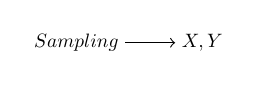
\begin{tikzpicture}[scale=0.8,every node/.style={scale=0.7},font=\tt]
    \node (Sampling) at ( 0, 0) {$Sampling$}; 
    \node (XY) at ( 2, 0) {$X,Y$};
%    \node (p3) at ( 0,-1) {$p_3$};
%    \node (p4) at ( 0,-2) {$p_4$};
%    \node (p5) at ( 1,-2) {$p_5$};

    \begin{scope}[every path/.style={->}]
       \draw (Sampling) -- (XY);
%       \draw (p3) -- (p4); 
%       \draw (p1) -- (p5);
%       \draw (p2) -- (p4);
%       \draw (p2) -- (p5);
    \end{scope}  
\end{tikzpicture}	
}
\caption{Relations between sources of uncertainty, labelled as in section~\ref{sec:sources}.}\label{fig:relations}
\end{figure}

%\begin{figure}[htb]
%\centering
%\resizebox{10cm}{!}{\input{Sources_uncertainty.tikz}}
%\caption{Relations between sources of uncertainty, labelled as in section~\ref{sec:sources}.}\label{fig:relations}
%\end{figure}


\section{Mathematical definitions of each, and their relations}

Equations, using content from e.g. \url{https://arxiv.org/abs/2109.12156} here showing how expected loss from each source of uncertainty would look like, and specifying any mathematical relations between them.


\section{Scope of our project}

Which sources of uncertainty will the way we will estimate uncertainty on performance metrics be included in our estimates?


\bibliographystyle{apalike} 
\bibliography{Sources_uncertainty}


\end{document}
